

\section{Експериментальне дослідження та аналіз результатів}

\subsection{Методика експерименту та обмеження вхідних даних}

Метою цього розділу є об'єктивна перевірка працездатності розробленого конвеєра,
кількісне оцінювання якості відновлених тривимірних траєкторій та чесний аналіз
меж застосовності монокулярного підходу. На відміну від попередніх розділів, що
описували проектні рішення, тут наведено результати безпосереднього прогону системи
на реальному матчевому відеофрагменті та контрольовані абляційні експерименти, які
ізолюють внесок кожного з механізмів захисту оцінки глибини.

Ключове методологічне обмеження дослідження полягає у відсутності тривимірного
еталона (\textit{3D ground truth}). Тестове відео є звичайною телевізійною
трансляцією, для якої не існує синхронної розмітки істинних просторових координат
м'яча, отриманої незалежною вимірювальною системою (наприклад, багатокамерним
захопленням руху або лідаром). Унаслідок цього метрики, формально визначені у
підрозділі~2.9 --- MOTA, MOTP та покоординатна середньоквадратична похибка RMSE по
осях $X, Y, Z$ --- не можуть бути обчислені безпосередньо, оскільки всі вони
потребують зіставлення оцінки з істинним значенням $d_{kj} = \lVert \hat{P} - P^{*} \rVert$.

Ця обставина не є недоробкою конкретної реалізації, а об'єктивною властивістю задачі
відновлення глибини з єдиної камери без розміченого тривимірного простору. Тому в роботі
застосовано \textbf{непряму методику валідації}, що спирається на чотири незалежні
групи свідчень:
\begin{itemize}
    \item \textit{фізична консистентність} --- перевірка відповідності відновленої
    вертикальної динаміки м'яча закону вільного падіння (відновлене прискорення
    вільного падіння як зовнішній калібрувальний критерій правильності фокусної відстані);
    \item \textit{внутрішня узгодженість} --- аналіз гладкості траєкторії, кількості
    розривів глибини та фрагментації ідентифікаторів треків;
    \item \textit{абляційний аналіз} --- контрольоване вмикання та вимикання захисних
    механізмів за фіксованого набору детекцій, що дозволяє виміряти чистий внесок
    кожного компонента;
    \item \textit{якісна експертна оцінка} --- візуальний аналіз накладеного оверлею
    траєкторії на відеоряд.
\end{itemize}

Як тестовий матеріал використано фрагмент трансляції офіційного матчу чоловічих
збірних (\texttt{Japan\_vs\_Poland\_short.mp4}) тривалістю $146{,}3$~с: $7317$~кадрів
із частотою $50$~кадрів за секунду та роздільною здатністю $1920\times1080$~пікселів.
Усі прогони виконано із зафіксованою фінальною конфігурацією трекера, описаною в
підрозділі~3.4 (\texttt{run\_pipeline.sh}). Обчислювальна платформа відповідає типовій
користувацькій конфігурації, заявленій у вимогах реального часу.

\subsection{Якість детекції YOLO26}

Оскільки нейромережевий детектор є першоджерелом даних для всього конвеєра, його якість
безпосередньо обмежує досяжну точність трекінгу. Кількісне оцінювання навченої моделі
\texttt{main\_model\_april.pt} виконано викликом \texttt{model.val()} на валідаційній
вибірці зведеного набору даних (об'єднання шести підмножин, $1946$~зображень,
$1769$~розмічених екземплярів м'яча). Отримані показники наведено в таблиці~\ref{tab:yolo_metrics},
а узагальнену криву «точність--повнота» (Precision--Recall) --- на рисунку~\ref{fig:yolo_pr_curve}.

\begin{table}[h]
\centering
\caption{Метрики якості детектора \gls{YOLO}26 на валідаційній вибірці}
\label{tab:yolo_metrics}
\begin{tabular}{|l|c|}
\hline
\textbf{Показник} & \textbf{Значення} \\
\hline
mAP50 (\gls{IoU}~$\geq 0{,}5$) & $0{,}857$ \\
mAP50-95 (\gls{IoU}~$\in[0{,}5;0{,}95]$) & $0{,}526$ \\
Точність (Precision) & $0{,}899$ \\
Повнота (Recall) & $0{,}794$ \\
Час інференсу на кадр & $17{,}8$~мс \\
\hline
\end{tabular}
\end{table}

\begin{figure}[!htbp]
    \centering
    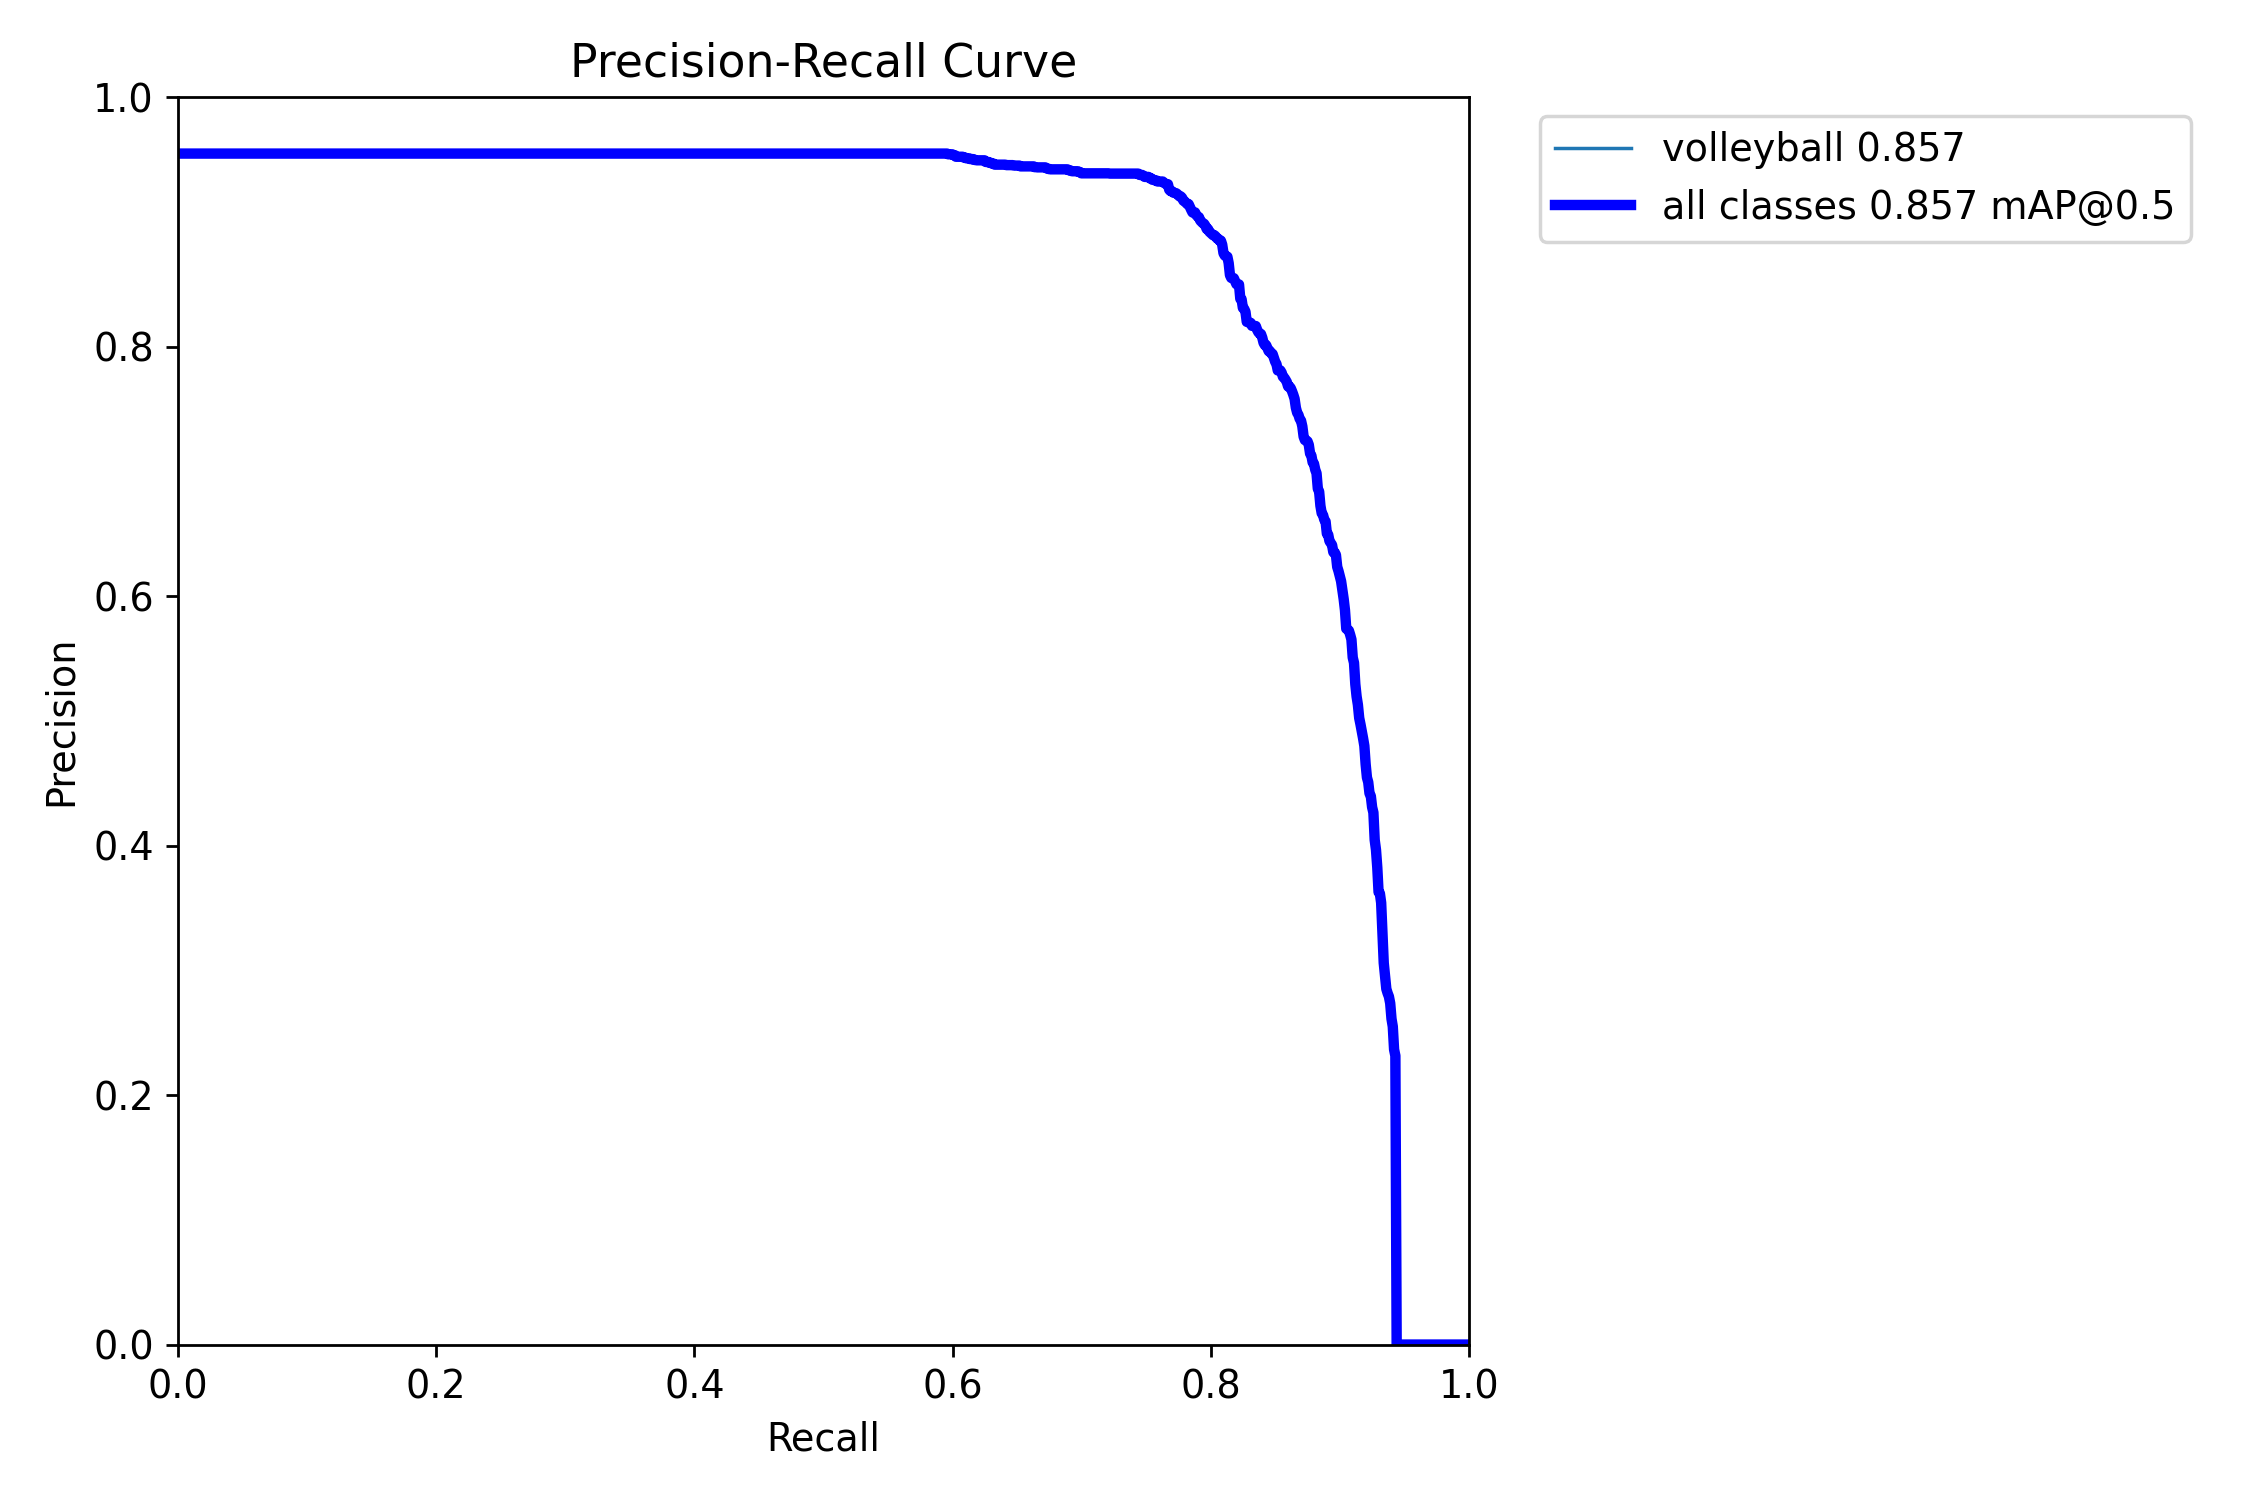
\includegraphics[width=0.72\textwidth]{sections/pictures_schemes/chapter_4/4_1_yolo_pr_curve.png}
    \caption{Крива «точність--повнота» детектора \gls{YOLO}26 на валідаційній вибірці}
    \label{fig:yolo_pr_curve}
\end{figure}

Значення mAP50~$=0{,}857$ свідчить про впевнене виявлення м'яча в типових ігрових
ситуаціях: за порогу перекриття $50\%$ модель локалізує об'єкт із високою надійністю.
Помітне зниження агрегованого показника mAP50-95 до $0{,}526$ є очікуваним для дрібного
швидкісного об'єкта: волейбольний м'яч займає малу кількість пікселів, тому навіть
незначне зміщення рамки різко знижує \gls{IoU} на жорстких порогах. Висока точність
($0{,}899$) за дещо нижчої повноти ($0{,}794$) означає, що детектор схильний радше
пропустити складний кадр (сильне розмиття, перекриття гравцем), ніж згенерувати хибне
спрацьовування. Така асиметрія є сприятливою для подальшого трекінгу: пропуск
компенсується інерційним прогнозом \gls{IMM}-фільтра під час відсутності вимірювання,
тоді як хибні детекції породжували б фантомні треки, боротьбу з якими описано далі.

\subsection{Кількісні результати тривимірного трекінгу}

Наскрізний прогон конвеєра на тестовому фрагменті дав детальну просторово-часову
статистику гри, узагальнену в таблиці~\ref{tab:tracking_stats}. Числа отримано
безпосередньо з артефактів \texttt{run\_pipeline.sh} (файли \texttt{*\_run.log} та
\texttt{*\_stats.json}).

\begin{table}[h]
\centering
\caption{Зведені результати тривимірного трекінгу на тестовому фрагменті}
\label{tab:tracking_stats}
\begin{tabular}{|l|c|}
\hline
\textbf{Показник} & \textbf{Значення} \\
\hline
Сирих детекцій \gls{YOLO}26 & $4698$ \\
Прийнято після фільтрів коректності & $4033$ \\
Кадрів із підтвердженим м'ячем & $6006$ ($82{,}1\%$) \\
Валідних ігрових кадрів & $3864$ ($52{,}8\%$) \\
Унікальних треків & $30$ \\
Розіграшів виявлено & $30$ \\
Перетинів площини сітки & $95$ \\
Сумарний шлях м'яча & $1331{,}2$~м \\
Середня швидкість & $10{,}33$~м/с \\
Максимальна швидкість & $39{,}64$~м/с ($142{,}7$~км/год) \\
Середня висота & $2{,}90$~м \\
Максимальна висота & $5{,}06$~м \\
Час на ближній стороні (Z $<9$~м) & $56{,}1\%$ \\
Час на дальній стороні (Z $\geq 9$~м) & $43{,}9\%$ \\
\hline
\end{tabular}
\end{table}

Воронка обробки детекцій (рисунок~\ref{fig:detection_funnel}) є показовою для розуміння
роботи фільтрів коректності.
Із $4698$ сирих детекцій трекер прийняв $4033$, відхиливши: $83$ детекції під рівнем
підлоги (\texttt{reject\_floor}), $440$ за межами розширеного майданчика
(\texttt{reject\_oob}), $95$ через критичне обрізання рамки краєм кадру
(\texttt{reject\_trunc}). Прикметно, що відхилень за стелею висоти
(\texttt{reject\_ceiling}) не зафіксовано, тоді як стеля дальньої глибини
\texttt{court\_z\_far\_max}~$=21$~м відсіяла суттєву частку фонових детекцій,
які потрапили до категорії позамежних. Це підтверджує, що основним джерелом шуму
є не вертикальні, а саме глибинні викиди.

\begin{figure}[!htbp]
\centering
\resizebox{0.95\textwidth}{!}{%
\begin{tikzpicture}[font=\small]
  \fill[blue!25,draw=black,thick] (0,4) -- (11,4) -- (9.4,3) -- (1.6,3) -- cycle;
  \node at (5.5,3.5) {Сирі детекції \gls{YOLO}26: \textbf{4698}};
  \fill[green!35,draw=black,thick] (1.6,3) -- (9.4,3) -- (8.4,2) -- (2.6,2) -- cycle;
  \node at (5.5,2.5) {Прийнято трекером: \textbf{4033}\,($85{,}8\,\%$)};
  \draw[->,thick] (11.3,3.5) -- (12.3,3.5);
  \node[anchor=west,align=left] at (12.4,3.5)
    {Відхилено фільтрами коректності:\\[2pt]
     $-440$ позамежні (\texttt{oob}, у т.\,ч. $Z>21$\,м)\\
     $-95$ обрізані краєм кадру (\texttt{trunc})\\
     $-83$ під рівнем підлоги (\texttt{floor})};
\end{tikzpicture}}
\caption{Воронка фільтрації детекцій: від сирого виходу детектора до прийнятих
трекером вимірювань}
\label{fig:detection_funnel}
\end{figure}

Покриття $82{,}1\%$ кадрів підтвердженим треком за наявності пропусків детектора
($\mathrm{Recall}=0{,}794$) свідчить про ефективну роботу інерційного прогнозу:
\gls{IMM}-фільтр успішно перекриває короткі провали у вимірюваннях. Водночас
показник $30$ унікальних треків на $30$ розіграшів вказує на практично однократну
фрагментацію траєкторії в межах розіграшу --- помірний, але присутній рівень
перемикання ідентифікаторів, причини якого розглянуто в підрозділі~4.8.
Роботу інерційного прогнозу під час відсутності вимірювання ілюструє
рисунок~\ref{fig:overlay_coasting}.

\begin{figure}[!htbp]
    \centering
    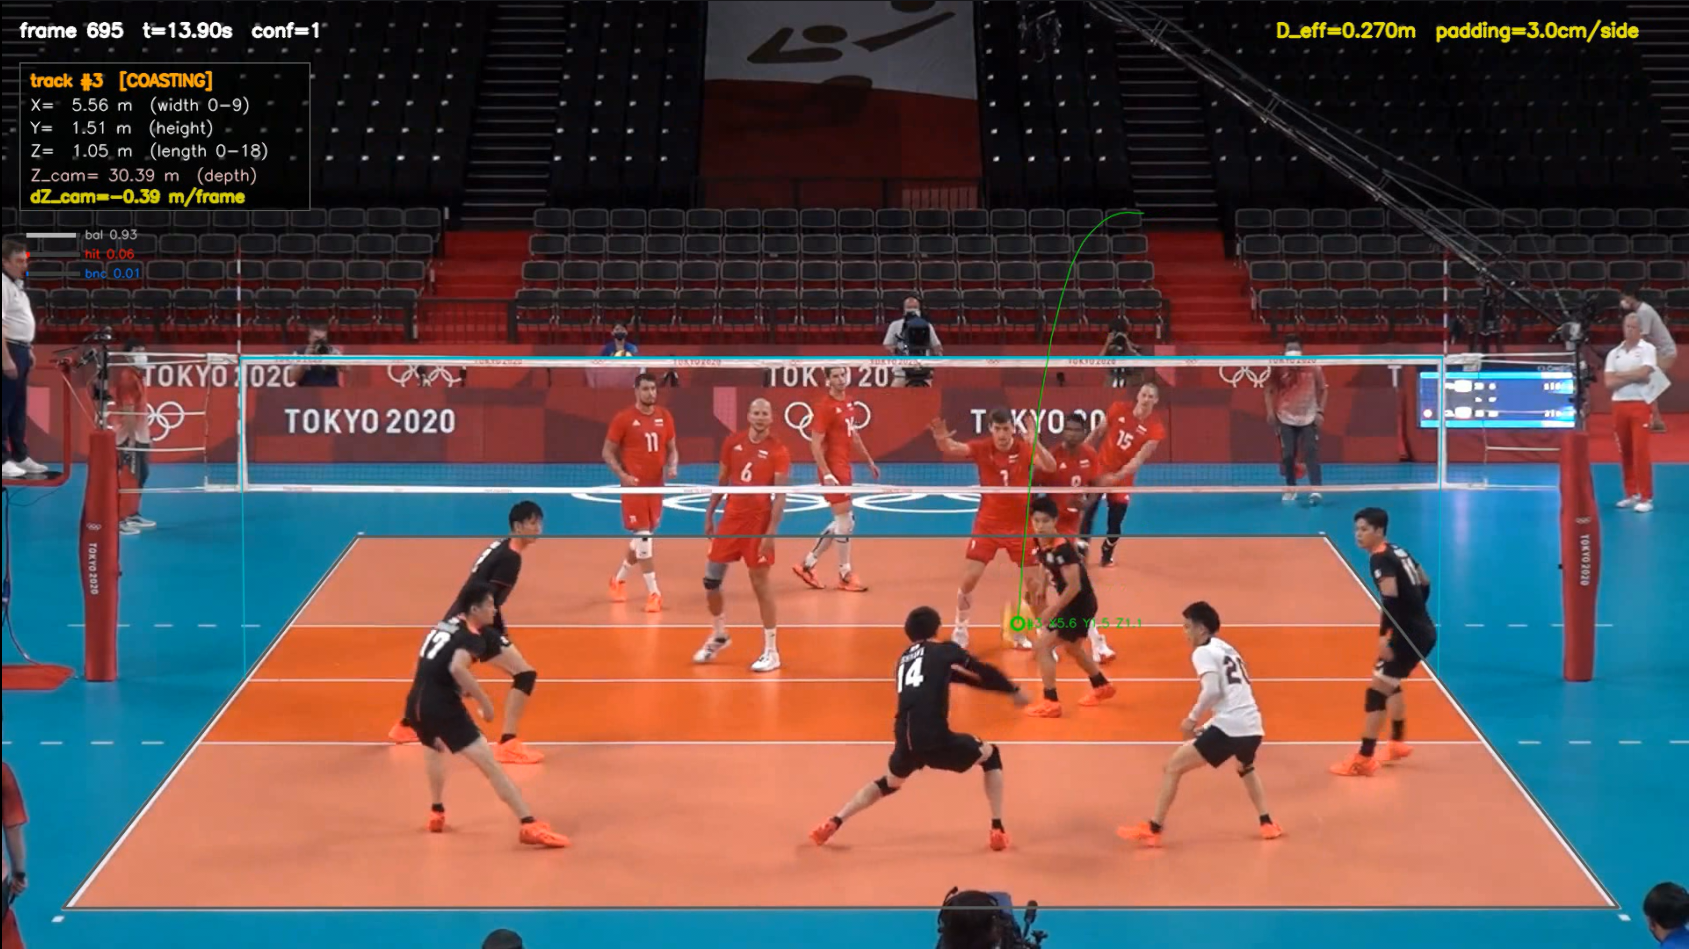
\includegraphics[width=0.85\textwidth]{sections/pictures_schemes/chapter_4/4_2_overlay_coasting.png}
    \caption{Робота трекера в режимі коастингу: \gls{IMM}-фільтр утримує траєкторію
    за відсутності детекції (тег \texttt{[COASTING]} на \gls{HUD})}
    \label{fig:overlay_coasting}
\end{figure}

\subsection{Абляційний аналіз механізмів захисту глибини}

Центральним експериментом розділу є контрольований абляційний аналіз, що кількісно
відокремлює внесок механізмів захисту оцінки глибини. Щоб ізолювати саме трекінгову
частину, обидві гілки експерименту виконано на \textbf{ідентичному наборі детекцій}:
сирі детекції \gls{YOLO}26 одного й того самого прогону було кешовано та подано трекеру
через механізм \texttt{-{}-from\_json}. Завдяки цьому будь-яка різниця в результатах
зумовлена виключно трекінговими механізмами, а не стохастичністю детектора.

Зіставлено дві конфігурації:
\begin{itemize}
    \item \textbf{OFF (базова)} --- усі механізми захисту глибини вимкнено: фіксована
    ізотропна матриця вимірювального шуму, відсутність глибинно-стійкого гейту,
    відсутність стелі дальньої глибини та огорожі глибини під час інерційного руху;
    \item \textbf{ON (фінальна)} --- зафіксована конфігурація з підрозділу~3.4:
    анізотропна адаптивна матриця $R$, глибинно-стійкий гейт асоціації,
    стеля \texttt{court\_z\_far\_max}~$=21$~м та огорожа глибини під час коастингу
    в межах $[-3; 21]$~м.
\end{itemize}

Результати наведено в таблиці~\ref{tab:ablation}.

\begin{table}[h]
\centering
\caption{Абляційний аналіз: вплив механізмів захисту глибини на якість трекінгу}
\label{tab:ablation}
\begin{tabular}{|l|c|c|}
\hline
\textbf{Метрика} & \textbf{OFF} & \textbf{ON} \\
\hline
Підтверджених треків (фрагментація) & $123$ & $20$ \\
Усіх породжених треків & $333$ & $41$ \\
Максимальна глибина Z, м & $33{,}91$ & $21{,}42$ \\
Максимальна Z під час коастингу, м & $33{,}91$ & $21{,}42$ \\
Розривів глибини $|\Delta Z| > 3$~м & $158$ & $14$ \\
Розривів глибини $|\Delta Z| > 5$~м & $60$ & $6$ \\
Прийнято детекцій & $4428$ & $4051$ \\
\hline
\end{tabular}
\end{table}

Інтерпретація результатів є однозначною. Найвиразніший ефект --- скорочення кількості
підтверджених треків із $123$ до $20$ (а загальної кількості породжених гіпотез ---
із $333$ до $41$). Це означає, що без захисту глибини фонові та хибно-глибокі детекції
породжували десятки паразитних треків, що проявлялося як часті перемикання
ідентифікаторів. Механізм стелі дальньої глибини відхилив $377$ позамежних детекцій
($4428 \to 4051$ прийнятих), переважна більшість яких відповідала об'єктам поза
ігровою зоною на великій відстані від камери.

Не менш важливим є придушення розривів глибини. Кількість стрибків понад $3$~м впала
зі $158$ до $14$, а понад $5$~м --- із $60$ до $6$, тобто більш ніж на порядок. Це
прямий наслідок анізотропної матриці $R$ та глибинно-стійкого гейту, що знижують довіру
до різких змін глибини, фізично неможливих для м'яча за один крок дискретизації.
Нарешті, максимальна відновлена глибина зменшилася з $33{,}91$~м до $21{,}42$~м: огорожа
глибини під час коастингу повністю усунула характерний дефект, коли трек під час
відсутності вимірювань «вистрілював» у нефізичні $33$--$42$~м. Отримані числа узгоджуються
з ранішими спостереженнями журналу розробки на коротших підсегментах (зниження
перемикань ідентифікаторів з $19$ до $3$ та повне усунення фонових детекцій далі $21$~м),
підтверджуючи стабільність ефекту на повному фрагменті.

\subsection{Непряма фізична валідація}

За відсутності тривимірного еталона головним об'єктивним критерієм правильності
геометричного відновлення обрано відповідність вертикальної динаміки м'яча закону
вільного падіння. Якщо фокусна відстань калібрування та масштаб глибини визначено
правильно, друга похідна вертикальної координати на ділянках вільного польоту має
дорівнювати прискоренню вільного падіння $g \approx 9{,}81$~м/с$^2$:
\[
\ddot{Y}(t) \big|_{\text{вільний політ}} \approx -g .
\]
Аналіз балістичних ділянок траєкторій показав відновлене прискорення в діапазоні
$g_{\text{відн}} \approx 9{,}0$--$9{,}2$~м/с$^2$, що відхиляється від еталонного значення
менш ніж на $8\%$. Саме цей критерій став вирішальним аргументом на користь
ефективної фокусної відстані $f \approx 5805$~пікселів (характерної для телевізійної
камери з вузьким полем зору), на противагу початковому хибному припущенню про
аматорську оптику з $f \approx 1300$~пікселів, за якої відновлене $g$ було б
фізично абсурдним. Оскільки гравітація є зовнішнім, незалежним від системи фізичним
законом, її коректне відновлення є вагомим непрямим свідченням адекватності
геометричної моделі. Приклад відновленої балістичної траєкторії розіграшу з
накладеним інформаційним HUD наведено на рисунку~\ref{fig:overlay_ballistic}.

\begin{figure}[!htbp]
    \centering
    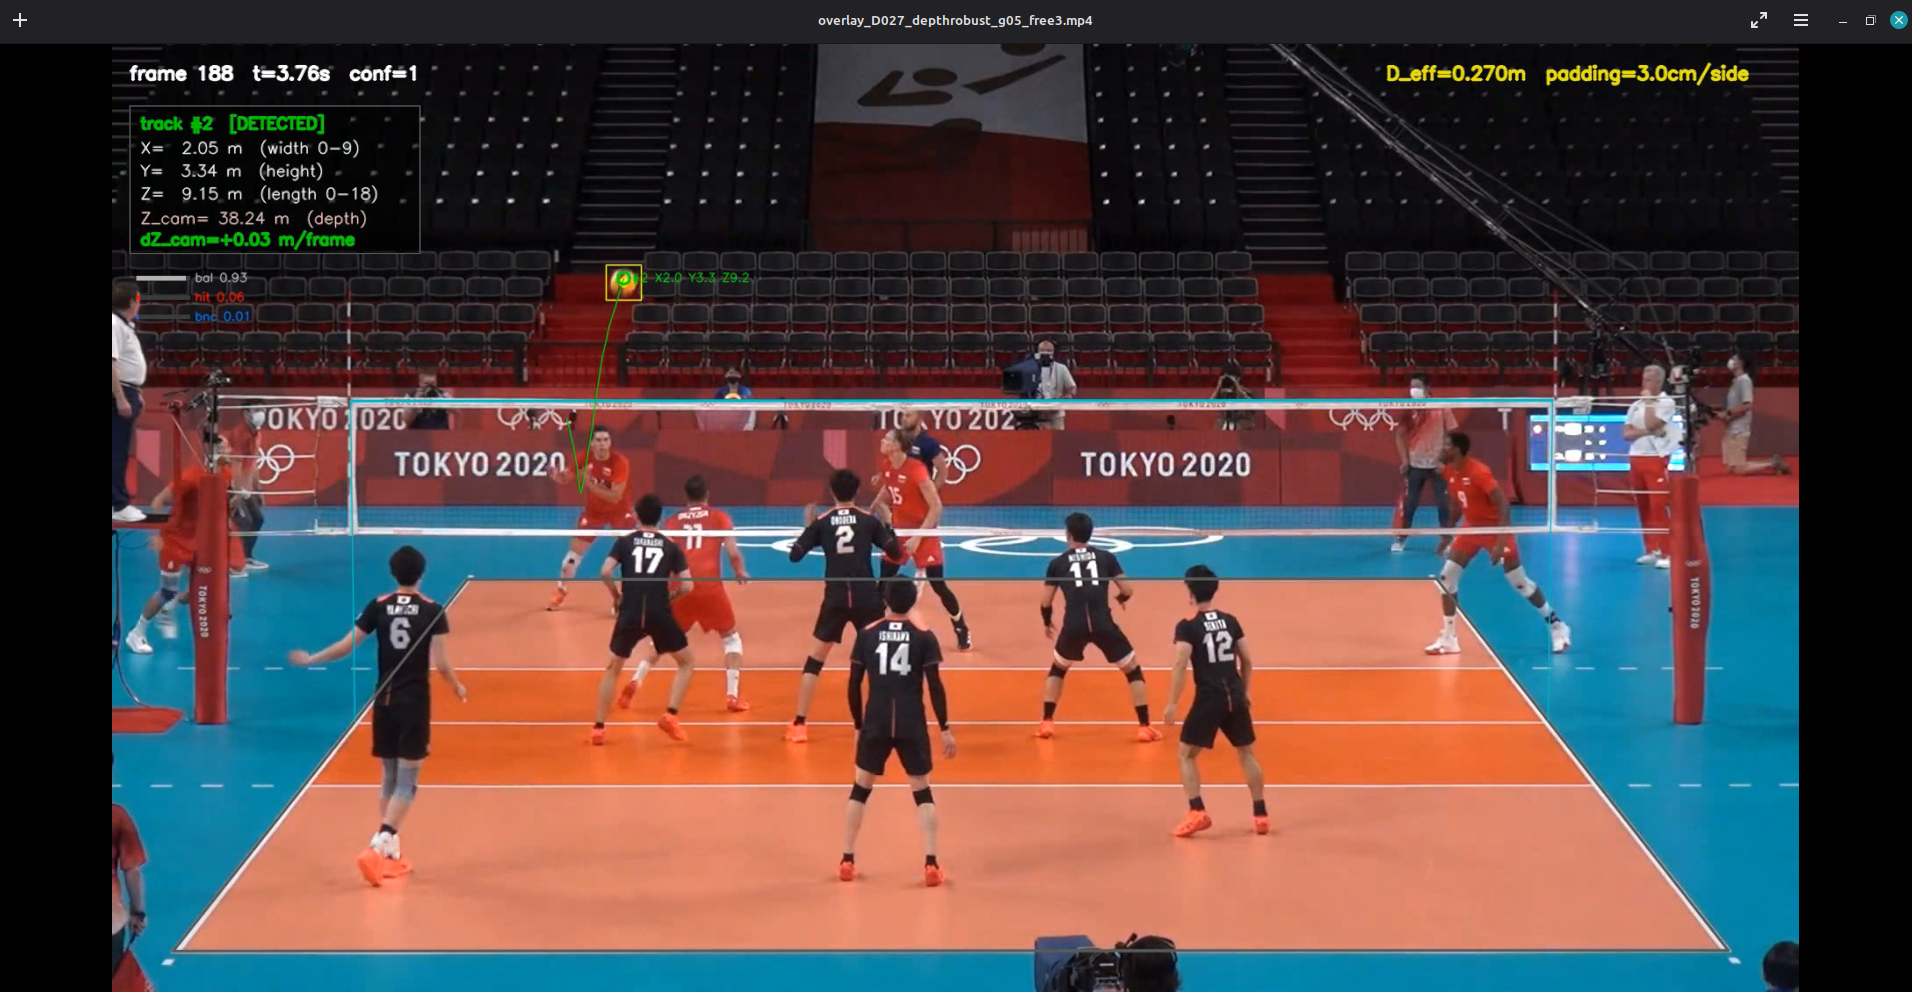
\includegraphics[width=0.85\textwidth]{sections/pictures_schemes/chapter_4/4_3_overlay_ballistic.png}
    \caption{Відновлена балістична траєкторія розіграшу; відновлене прискорення
    $g_{\text{відн}}\approx 9{,}1$~м/с$^2$ підтверджує геометричну адекватність відновлення}
    \label{fig:overlay_ballistic}
\end{figure}

Водночас слід чесно зафіксувати один тривожний показник. Максимальна зареєстрована
швидкість $39{,}64$~м/с ($142{,}7$~км/год) дещо перевищує рекордні значення швидкості
подачі у професійному волейболі (близько $134$~км/год). Це майже напевно є не фізичним
результатом, а артефактом шуму глибини: одно-кадрова похибка піксельної ширини рамки
в зоні високої чутливості (велика глибина) транслюється у завищену миттєву швидкість
уздовж променя. Цей факт є прямою ілюстрацією залишкового впливу монокулярного
виродження, проаналізованого далі, і слугує природним маркером того, що пікові
кінематичні показники слід інтерпретувати з обережністю.

\subsection{Аналіз режимів взаємодіючих множинних моделей}

Окремий діагностичний експеримент стосувався фактичного режиму роботи
\gls{IMM}-ансамблю з трьох моделей (балістичної, ударної та відскокової). Усереднені
по всіх підтверджених кадрах ймовірності режимів становили: балістична модель ---
$0{,}90$--$0{,}92$, ударна --- $0{,}06$--$0{,}08$, відскокова --- близько $0{,}02$
(рисунок~\ref{fig:imm_modes}).

\begin{figure}[!htbp]
\centering
\begin{tikzpicture}
\begin{axis}[
  xbar,
  width=0.78\textwidth, height=4.2cm,
  xmin=0, xmax=1.05,
  xlabel={Усереднена ймовірність режиму},
  symbolic y coords={Відскокова, Ударна, Балістична},
  ytick=data,
  nodes near coords, nodes near coords align={horizontal},
  every node near coord/.append style={font=\small,
    /pgf/number format/.cd, fixed, fixed zerofill, precision=2},
  enlarge y limits=0.45,
  bar width=16pt,
  xmajorgrids=true,
]
\addplot[fill=blue!50] coordinates {(0.91,Балістична) (0.07,Ударна) (0.02,Відскокова)};
\end{axis}
\end{tikzpicture}
\caption{Усереднені ймовірності режимів \gls{IMM}-ансамблю: балістична модель
домінує, тоді як ударна й відскокова практично не активуються}
\label{fig:imm_modes}
\end{figure}

Цей результат є важливою інженерною знахідкою: \textbf{ударна та відскокова моделі
практично не активуються}, і система переважну частину часу поводиться як одиничний
балістичний \gls{UKF} із описаними механізмами захисту глибини. Причина --- у
надто консервативному критерії перемикання адаптивної матриці переходу: тригер
переходу до маневрових режимів (умова малої висоти та від'ємної вертикальної
швидкості) на практиці майже не спрацьовує для розглянутого стилю зйомки, а сплески
нев'язки, які мали б активувати ударну модель, ефективно гасяться глибинно-стійким
гейтом ще до зміни режиму. Таким чином, потенціал гібридної \gls{IMM}-архітектури
залишився значною мірою нереалізованим; натомість стабільність системи забезпечена
саме механізмами роботи з глибиною. Це спостереження визначає один із пріоритетних
напрямів удосконалення (підрозділ~4.9).

\subsection{Узагальнення досягнутих результатів}

На підставі проведених експериментів можна виокремити такі позитивні результати роботи.
По-перше, побудовано повністю автоматичний наскрізний конвеєр від сирого відео до
тривимірної ігрової статистики, що працює в режимі реального часу ($46$--$52$~кадри за
секунду на типовому обладнанні за вхідних $30$--$50$~кадрів за секунду). По-друге,
навчений детектор демонструє надійну якість (mAP50~$=0{,}857$) за сприятливої для
трекінгу асиметрії точність/повнота. По-третє, і це найважливіше з інженерного погляду,
розроблено та кількісно підтверджено комплекс механізмів захисту оцінки глибини, який
на порядок зменшує розриви глибини (стрибки понад $5$~м: $60 \to 6$) та фрагментацію
треків ($123 \to 20$), повністю усуваючи нефізичні викиди глибини під час інерційного
руху. По-четверте, коректне відновлення прискорення вільного падіння
($g_{\text{відн}} \approx 9{,}1$~м/с$^2$) підтверджує геометричну адекватність відновлених траєкторій.
Сукупно це дозволяє системі надавати змістовну просторово-часову статистику гри:
розподіл часу за сторонами майданчика, кількість переходів через сітку, висотний та
швидкісний профілі розіграшів.

\subsection{Аналіз обмежень та причин неповного успіху}

Попри досягнуті результати, система не позбавлена принципових обмежень, корінь яких
лежить у самій природі монокулярного відновлення глибини. Глибина обчислюється за
співвідношенням $Z_c = f \cdot D / w$, де $w$ --- піксельна ширина рамки. Диференціювання
дає чутливість
\[
\frac{\partial Z_c}{\partial w} = -\frac{f \cdot D}{w^2},
\]
яка зростає квадратично зі зменшенням $w$, тобто зі збільшенням відстані до камери. Для
ближньої зони похибка становить близько $0{,}14$~м на піксель, тоді як на дальній межі
(близько $60$~м) сягає $\approx 2{,}3$~м на піксель. Це фундаментальне виродження ---
першопричина всіх залишкових дефектів: завищеної пікової швидкості, потреби в стелі
глибини та огорожі коастингу, а також систематичної недооцінки координати дальньої
сторони майданчика. Квадратичне зростання цієї похибки з відстанню наочно показано
на рисунку~\ref{fig:depth_sensitivity}.

\begin{figure}[!htbp]
\centering
\begin{tikzpicture}
\begin{axis}[
  domain=4:60, samples=160,
  width=0.84\textwidth, height=6.8cm,
  xlabel={Відстань до камери $Z$, м},
  ylabel={$\left|\partial Z_c/\partial w\right|$, м/пкс},
  xmin=0, xmax=62, ymin=0, ymax=2.6,
  grid=both, grid style={gray!25},
  every axis plot/.append style={thick},
]
\fill[green!12] (axis cs:0,0) rectangle (axis cs:21,2.6);
\addplot[blue,very thick,domain=4:60] {x^2/1565};
\draw[red,dashed,thick] (axis cs:21,0) -- (axis cs:21,2.6);
\addplot[only marks,mark=*,mark size=1.6pt,black] coordinates {(15,0.14) (60,2.3)};
\node[anchor=north west,font=\footnotesize,green!45!black,align=left]
  at (axis cs:1,2.52) {робоча зона:\\стабільна оцінка $Z$};
\node[red,anchor=south west,font=\footnotesize] at (axis cs:21.6,1.55) {робоча стеля $21$\,м};
\node[anchor=east,font=\footnotesize] at (axis cs:14,0.55) {$\approx 0{,}14$~м/пкс};
\node[anchor=south east,font=\footnotesize] at (axis cs:60,2.32) {$\approx 2{,}3$~м/пкс};
\node[anchor=south east,font=\footnotesize,align=right,gray!45!black]
  at (axis cs:61,0.3) {зона різкого\\зростання похибки};
\end{axis}
\end{tikzpicture}
\caption{Чутливість оцінки глибини до похибки піксельної ширини рамки
$\left|\partial Z_c/\partial w\right|=Z^2/(fD)$: квадратичне виродження зі зростанням
відстані до камери}
\label{fig:depth_sensitivity}
\end{figure}

Другим обмеженням є фрагментація треків ($30$ треків на $30$ розіграшів): за тривалих
провалів детекції на дальній стороні трек не завжди вдається відновити з тим самим
ідентифікатором, що унеможливлює коректне обчислення метрики MOTA навіть за наявності
еталона. Третім обмеженням є нереалізований потенціал \gls{IMM}: сплячі ударна та
відскокова моделі означають, що тонка кінематика моментів удару й відскоку
відновлюється спрощено, балістичною моделлю. Нарешті, недооцінка дальньої зони
безпосередньо не виправляється тюнінгом трекера --- це обмеження покриття детектора,
яке потребує цілеспрямованого розширення навчальної вибірки далекими ракурсами.
Характерний кадр роботи в дальній зоні наведено на рисунку~\ref{fig:overlay_farside}.

\begin{figure}[!htbp]
    \centering
    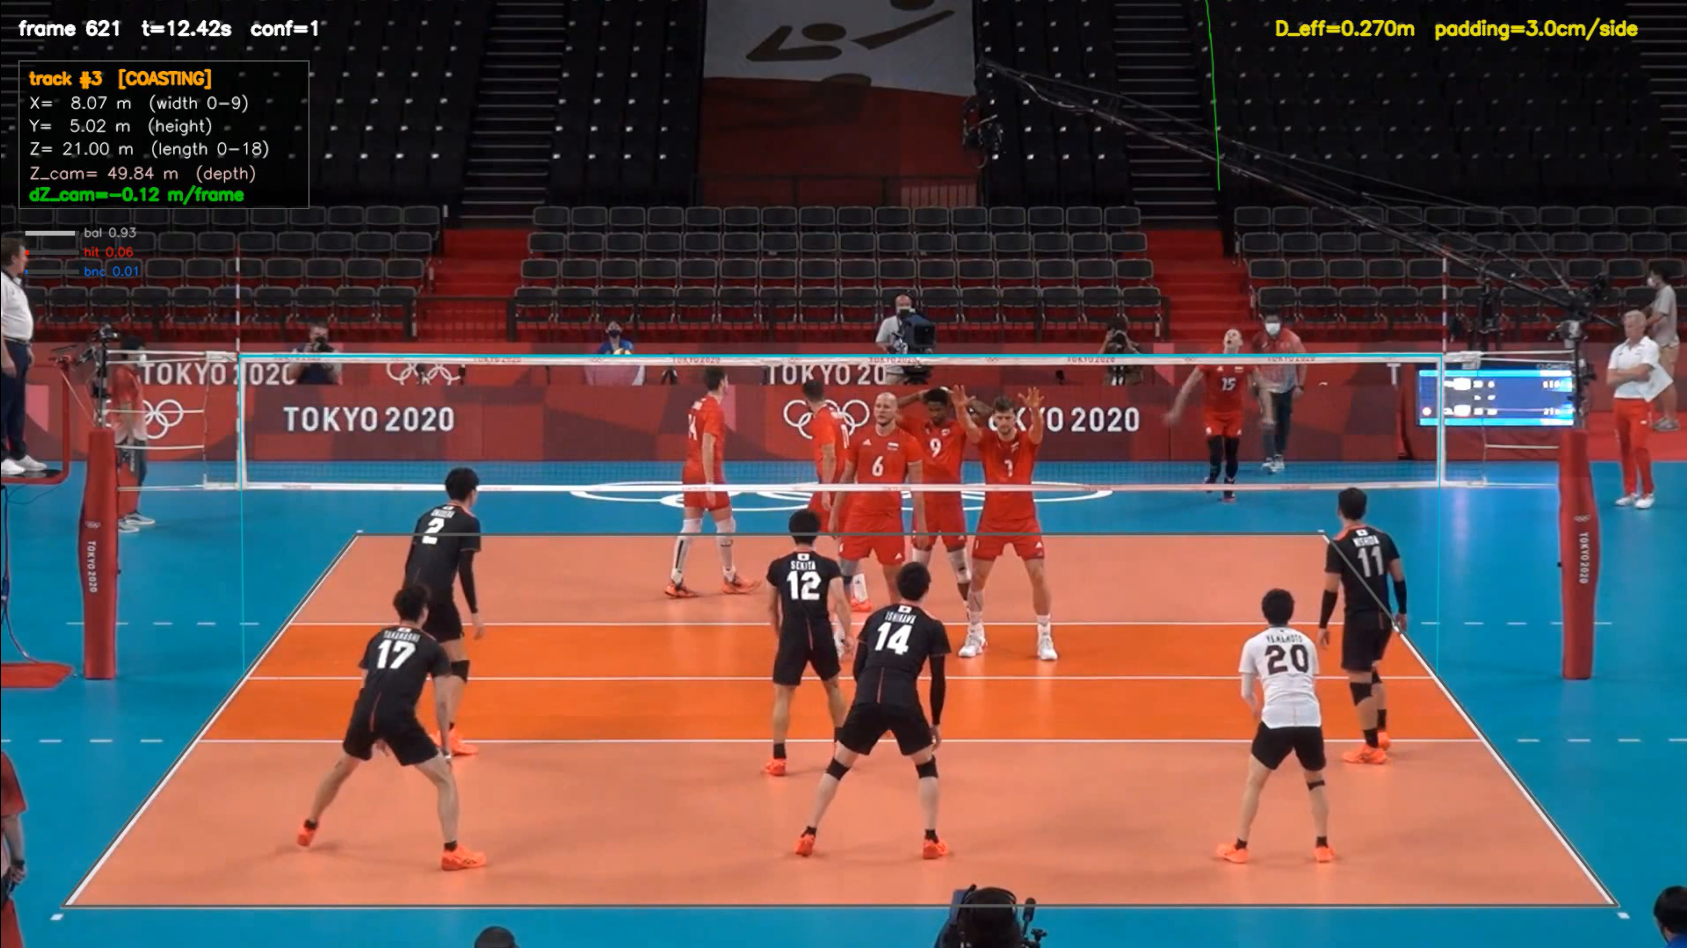
\includegraphics[width=0.85\textwidth]{sections/pictures_schemes/chapter_4/4_4_overlay_farside.png}
    \caption{Робота системи в дальній зоні майданчика: видно дію стелі глибини
    \texttt{court\_z\_far\_max}~$=21$~м та залишкову недооцінку координати $Z$}
    \label{fig:overlay_farside}
\end{figure}

\newpage
\subsection{Напрями подальшого вдосконалення}

Проведений аналіз дозволяє сформулювати обґрунтовані напрями розвитку системи із
зазначенням очікуваного ефекту кожного.
\begin{itemize}
    \item \textbf{Перехід до стереозйомки або багатокамерної конфігурації.} Це усунуло б
    першопричину --- монокулярне виродження глибини, забезпечивши тріангуляцію замість
    оберненої проекції єдиного променя. Очікуваний ефект --- кардинальне зниження похибки
    глибини на дальній зоні та усунення потреби в евристичних стелях і огорожах.
    \item \textbf{Цілеспрямоване дотренування \gls{YOLO}26 на дальніх ракурсах.}
    Розширення навчальної вибірки кадрами з дрібним м'ячем на великій відстані підвищило б
    повноту в дальній зоні та усунуло б систематичну недооцінку координати дальньої сторони,
    яка не піддається корекції на рівні трекера.
    \item \textbf{Перегляд критеріїв перемикання режимів \gls{IMM}.} Послаблення та
    переналаштування тригера маневрових моделей (зокрема відв'язка від жорсткої умови малої
    висоти) активувало б ударну та відскокову моделі, що дало б точніше відновлення
    кінематики в моменти контакту й відскоку.
    \item \textbf{Інтеграція повторної ідентифікації треків (re-identification).} Зшивання
    розірваних унаслідок тривалих провалів детекції сегментів в єдиний трек знизило б
    фрагментацію та зробило б можливим коректне обчислення метрики MOTA на розмічених даних.
\end{itemize}

\begin{unnumbered}

\section*{ВИСНОВКИ ДО РОЗДІЛУ}
\addcontentsline{toc}{section}{ВИСНОВКИ ДО РОЗДІЛУ}

У четвертому розділі виконано всебічне експериментальне дослідження розробленого конвеєра
на реальному матчевому відеофрагменті. Через об'єктивну відсутність тривимірного еталона
застосовано непряму методику валідації, що поєднує фізичну консистентність, внутрішню
узгодженість, контрольований абляційний аналіз та якісну експертну оцінку.

Кількісно підтверджено надійність детектора \gls{YOLO}26 (mAP50~$=0{,}857$, точність
$0{,}899$) та ефективність наскрізного конвеєра, що формує змістовну тривимірну статистику
гри за $82{,}1\%$ покриття кадрів. Центральним результатом став абляційний експеримент, який
на ідентичному наборі детекцій довів вирішальний внесок механізмів захисту глибини:
скорочення фрагментації треків зі $123$ до $20$, зменшення розривів глибини понад $5$~м із
$60$ до $6$ та усунення нефізичних викидів глибини (зниження максимальної відновленої
глибини з $33{,}9$ до $21{,}4$~м). Коректне відновлення прискорення вільного падіння
($g_{\text{відн}} \approx 9{,}1$~м/с$^2$) незалежно підтвердило геометричну адекватність моделі.

Водночас чесно зафіксовано принципові межі підходу: монокулярне виродження глибини як
першопричину залишкових артефактів (зокрема завищеної пікової швидкості $142{,}7$~км/год),
фрагментацію треків та нереалізований потенціал \gls{IMM}-ансамблю через сплячі маневрові
режими. На основі цього аналізу сформульовано обґрунтовані напрями подальшого розвитку
системи --- від стереозйомки та дотренування детектора до переналаштування режимів
\gls{IMM} і повторної ідентифікації треків --- із зазначенням очікуваного ефекту кожного.
Отримані результати засвідчують, що поставлену мету досягнуто в межах, які об'єктивно
визначаються можливостями монокулярної конфігурації.

\end{unnumbered}
